\textcolor{black}{\section{Introducción}}

\noindent La difracción de Bragg por rayos X tiene numerosas aplicaciones en la industria, sus usos van desde el control de calidad de semiconductores en donde su aplicación mejora la pureza de los semiconductores tales como el silicio, hasta en la minería en donde se utilizar para identificar los minerales presentes en distintas rocas. Los rayos X fueron descubiertos por accidente en el año 1895 por el físico Wilhelm Conrad Roentgen, por aquella época había muchos científicos interesados en los rayos catódicos y Wilhelm no era la excepción. Mientras experimentaba con un tubo de rayos X observó un papel pintado con una sustancia fluorescente. De inmediató intuyó que se encontró frente a algo totalmente nuevo. Pasó los próximos días estudiando estos rayos de forma tan minuciosa que tuvieron que pasar al menos 17 años para que se encontrara alguna característica nueva de estos. 

Años más tarde Max Von Laue en 1912, se le ocurrió hacer pasar estos rayos a través de cristales de sulfato de cobre. Y descubrió que se difractaban al igual que ocurría con la luz, esto le valió el Premio Nobel de Física en 1914. Identificó que estos rayos que hasta ese momento tenía una naturaleza desconocida, se trataban de nada mas y nada menos que ondas elentromagnéticas. 

Finalmente, William Lawrence Bragg y William Henry Bragg, determinaron que el patrón de difracción que Laue había identificado proporcionaba información acerca de la estructura interna  de los cristales sobre los que se incidían los rayos X. Henry y Lawrence plantearon la existencia de una especie de planos al interior de cristal, separados entre sí una distancia constante "d". Dichos planos serían capaz de reflejar la luz, cuando las ondas que indían sobre dos planos tuvieran una interferencia constructiva. Lawrence descubrió que las suma de las ondas de forma contructiva existiría únicamente cuando las ondas se encontratan en fase, y esto ocurre, cuando las ondas diferen estre sí un múltiplo entero de su longitud de onda. Así, plantearon lo que hoy se conoce como "La Ley de Bragg": 
\begin{equation}
	n\lambda = d\sin\theta
	\label{eq:bragg}
\end{equation}
Donde:
\begin{itemize}
	\item $d$ = distancia interplanar, \quad
	$n$ = orden de difracción, \quad
	$\lambda$ = longitud de onda, \quad
	$\theta$ = ángulo de Bragg.
\end{itemize}
Un cristal se puede entender como una arreglo periódico de átomos. Los sólidos cristalinos se caracterizan por presentar una distribución periódica y tridimensional de átomos, iones o grupos de átomos. Esta periodicidad se describe mediante una red cristalina, definida como un conjunto de puntos matemáticos equivalentes unidos por vectores de traslación, y una base, que corresponde al grupo de átomos asociado a cada punto de la red. La repetición de la base en todos los puntos de la red origina la estructura cristalina del material.

La unidad mínima que permite reproducir la estructura por traslación se denomina celda primitiva. En una celda primitiva existe un punto de red y su volumen corresponde al mínimo necesario para generar la totalidad del cristal. 
\begin{figure}
	\centering
	
\includegraphics[width=0.6\linewidth]{image.png}
	\caption{El área sombreada se trata de la celda primitiva}
	\label{fig:placeholder}
\end{figure}
Según las relaciones entre las longitudes de sus ejes y los ángulos que forman, las redes tridimensionales se clasifican en catorce redes de Bravais, agrupadas en siete sistemas cristalinos: triclínico, monoclínico, ortorrómbico, tetragonal, cúbico, trigonal y hexagonal. En particular, el sistema cúbico comprende las redes cúbica simple, cúbica centrada en el cuerpo y cúbica centrada en las caras.

Además de la distancia interplanar, la orientación de los planos cristalinos se
describe mediante los índices de Miller, denotados como $(hkl)$. Estos índices se
obtienen a partir de los interceptos que un plano forma con los ejes
cristalográficos $a_1$, $a_2$ y $a_3$. Para determinarlos, se expresan dichos
interceptos en unidades de las constantes de red, se calculan sus recíprocos y
se reducen a la menor relación de números enteros. Por ejemplo, para un plano
con interceptos $4a_1$, $a_2$ y $2a_3$, los recíprocos son
$1/4$, $1$ y $1/2$; al multiplicar por cuatro se obtienen los índices
$(142)$.

En los cristales cúbicos, algunos planos de especial importancia son $(100)$,
$(110)$, $(111)$ y $(200)$. El plano $(200)$ es paralelo al plano $(100)$. Los índices de Miller permiten relacionar los
picos observados en el patrón de difracción con familias específicas de planos atómicos dentro de la red cristalina.
\begin{figure}[H]
	\centering
	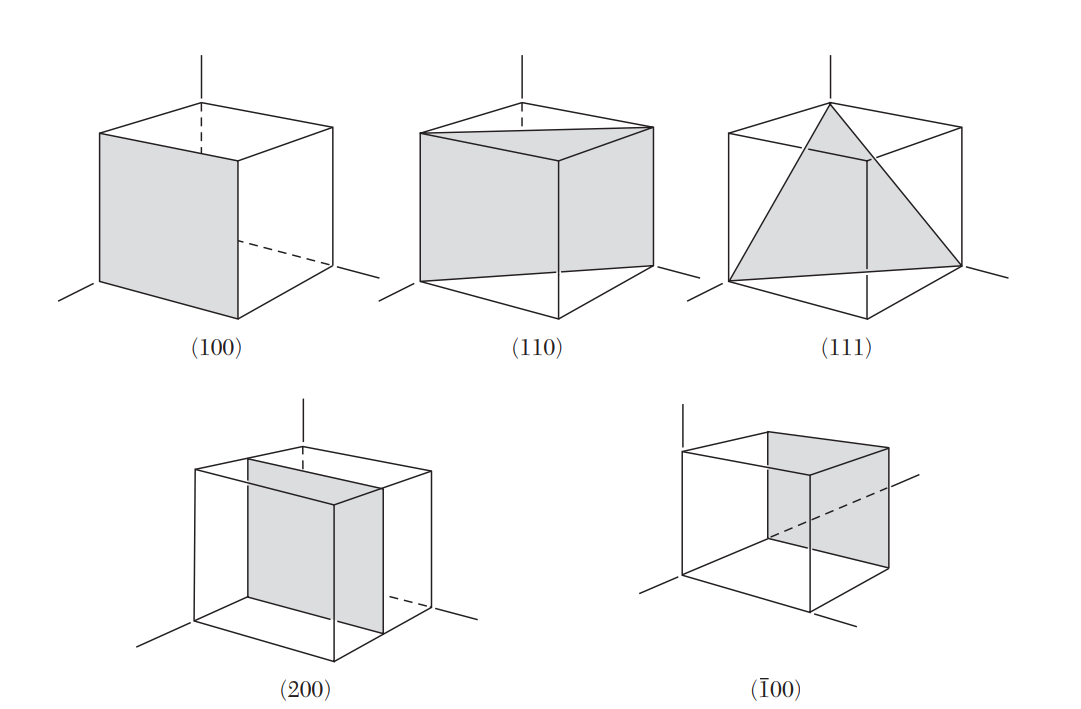
\includegraphics[width=0.5\linewidth]{figs/3.png}
	\caption{Planos más importantes para en un cristal cúbico}
	\label{fig:placeholder}
\end{figure}